\documentclass[10pt]{article}
\usepackage[margin=0.8in]{geometry}
\usepackage{graphicx,amsmath,amssymb,caption}
\captionsetup{font=small,labelfont=bf}
\graphicspath{{../../fig/gen/}}
\title{LaRC: figure candidates (real inference)}
\date{}
\begin{document}\maketitle
\noindent All panels come from the trained checkpoints on real T-LESS test crops (GT crops, LiePose protocol), 100k$\times$32 models,
EMA weights. ``LaRC'' is the joint model (82.2 AR); ``control'' has the same trained encoder and no world-model inputs. Crops in
Figs.~1--4 and 6 follow a fixed rule chosen before looking at outputs (first test crop per object with $\geq$25\% visible mask; objects 5, 8, 18,
21, 23, 27). CAD outlines are drawn for display only; LaRC never uses a mesh.

\begin{figure}[h]\centering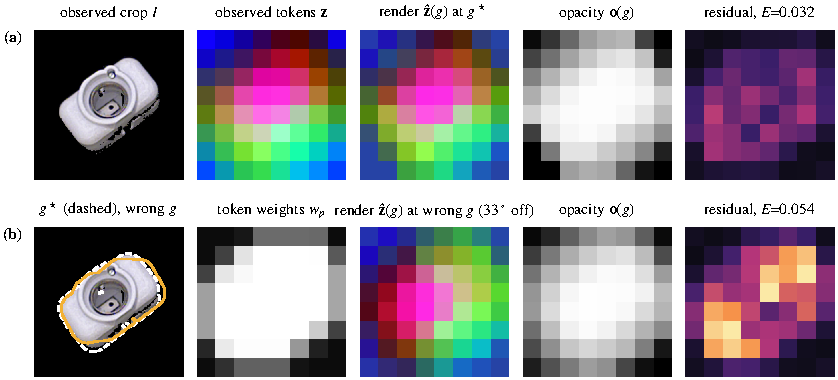
\includegraphics[width=\linewidth]{fig_render_compare.pdf}
\caption{\textbf{Render and compare.} (a) The observation, its comparison tokens (PCA to RGB, one basis per row pair), the field's
rendering at the ground-truth pose, its opacity, and the weighted residual: the rendering reproduces the observed tokens ($E=0.032$).
(b) A hypothesis the sampler visited, $33^\circ$ off in rotation with nearly the right translation: the residual concentrates where
the hypothesis places the wrong part of the object ($E=0.054$). Same colour scale in both rows.}\end{figure}

\begin{figure}[h]\centering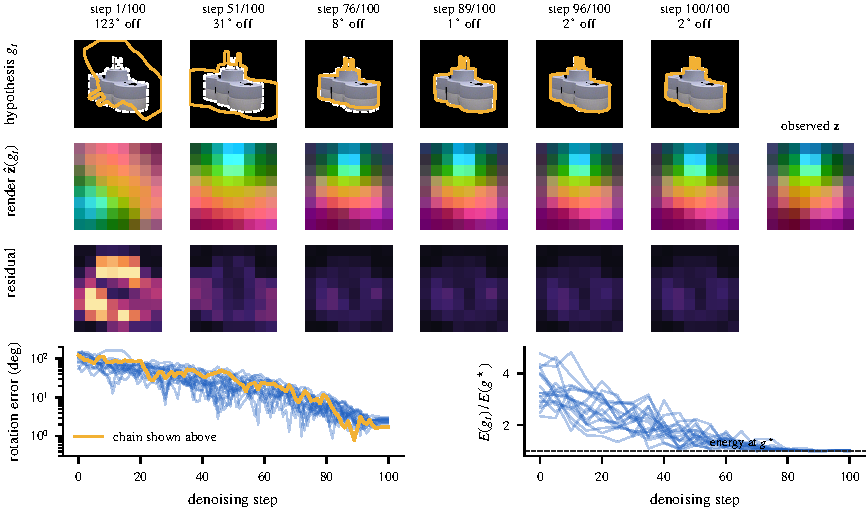
\includegraphics[width=\linewidth]{fig_in_loop.pdf}
\caption{\textbf{The comparison inside the loop.} One sampler chain for object 23: the hypothesis $g_t$ (orange outline; dashed: ground
truth), the field's rendering at $g_t$, and the residual, at six of the 100 steps. Bottom: rotation error and energy (relative to the
energy at $g^\star$) of all 16 chains from independent priors. The residual and the energy fall together as the chains converge.}\end{figure}

\begin{figure}[h]\centering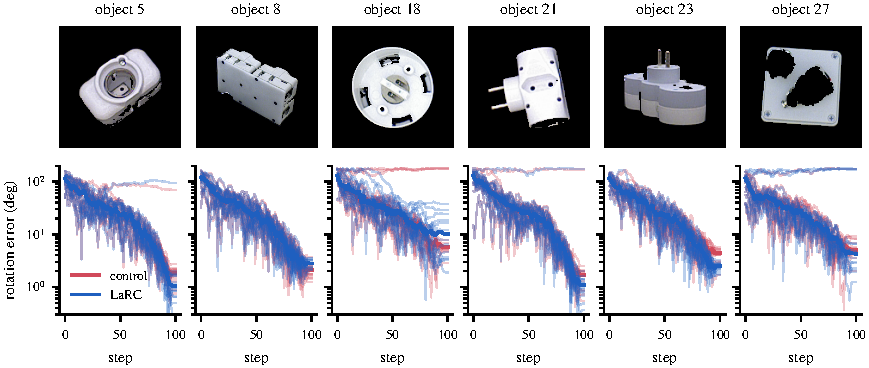
\includegraphics[width=\linewidth]{fig_trajectories.pdf}
\caption{\textbf{Sampler trajectories, LaRC vs.\ control}, same priors and noise, 16 chains per crop (thin) and their median (thick). On
these clearly visible crops both models converge; the gains of LaRC are on the harder part of the test set (Figs.~6, 7). Chains stuck
near $180^\circ$ are flipped near-symmetric modes.}\end{figure}

\begin{figure}[h]\centering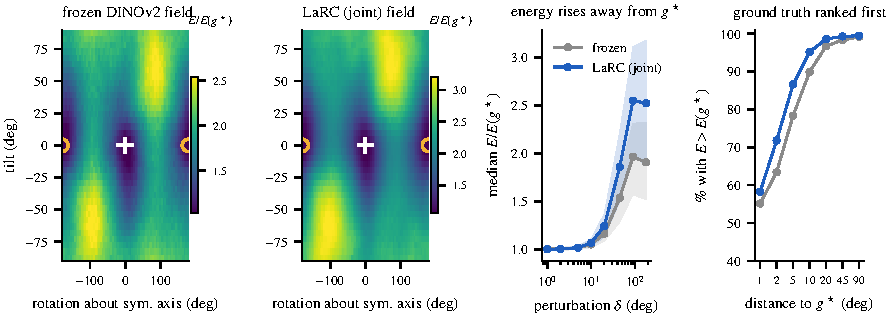
\includegraphics[width=\linewidth]{fig_energy.pdf}
\caption{\textbf{The energy.} Left: $E$ on a slice of $\mathrm{SO}(3)$ through the ground truth ($+$) and its symmetric copy
($\circ$, object 5), for the frozen-DINOv2 field and the jointly trained field; both poses have the same energy. Right, 400 random
test crops, 8 random axes each: the median energy ratio after rotating the ground truth by $\delta$ (band: interquartile range), and how
often a perturbed pose has higher energy than the ground truth, by its symmetry-aware distance. Joint training makes the energy
steeper (2.5$\times$ vs.\ 2.0$\times$ at $90^\circ$) and ranks the ground truth first more often (96\% vs.\ 93\% beyond $5^\circ$).}\end{figure}

\begin{figure}[h]\centering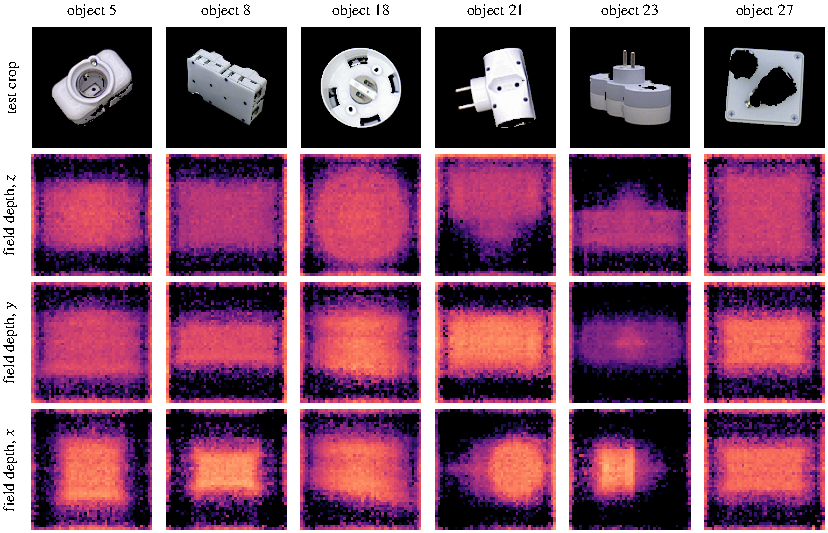
\includegraphics[width=0.75\linewidth]{fig_geometry.pdf}
\caption{\textbf{Shape emerges without supervision.} Depth at which rays along each object axis become 63\% opaque in the jointly trained
field (bright: near). The density is never supervised and the field never sees a mesh, yet the coarse shape of each object appears
(the disc of 18, the plug of 21, the three lobes of 23). The speckle is low-density fog in empty parts of the box.}\end{figure}

\begin{figure}[h]\centering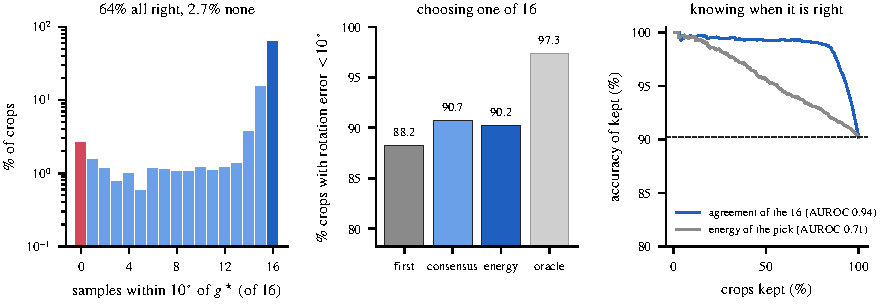
\includegraphics[width=\linewidth]{fig_selection.pdf}
\caption{\textbf{Many samples, one answer} (LaRC, all 6815 test crops, 16 samples each; correct: rotation error $<10^\circ$,
symmetry-aware). Left: in 64\% of crops all 16 samples are correct, in 2.7\% none. Middle: choosing one sample by consensus or lowest
energy recovers part of the gap to the oracle. Right: the agreement among the 16 samples is a strong confidence signal (AUROC 0.94);
the energy of the pick is weaker (0.71).}\end{figure}

\begin{figure}[h]\centering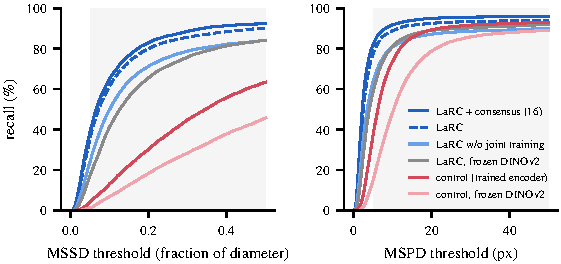
\includegraphics[width=0.7\linewidth]{fig_accuracy.pdf}
\caption{\textbf{Accuracy over the full test set}: recall as a function of the BOP MSSD and MSPD thresholds (shaded: the range BOP
averages). From the BOP evaluator's per-instance errors.}\end{figure}

\begin{figure}[h]\centering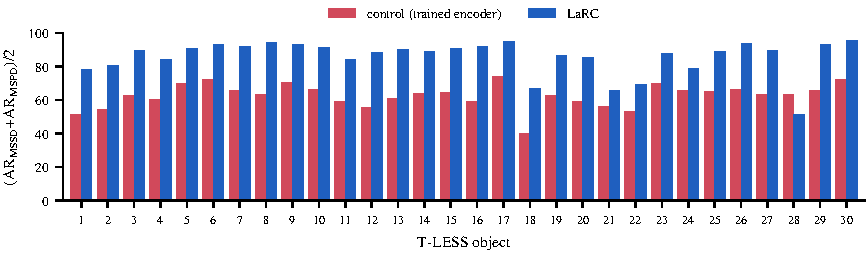
\includegraphics[width=\linewidth]{fig_per_object.pdf}
\caption{\textbf{Per object.} Mean of the MSSD and MSPD recalls over BOP thresholds, per T-LESS object. LaRC is better on 29 of 30
objects; object 28 is the exception.}\end{figure}

\begin{figure}[h]\centering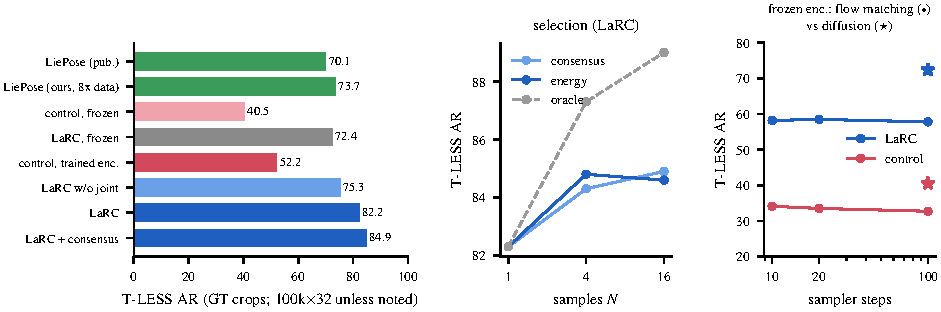
\includegraphics[width=\linewidth]{fig_summary.pdf}
\caption{\textbf{Results at a glance} (numbers from the paper's tables). Left: T-LESS AR. Middle: selection among $N$ samples.
Right: frozen-encoder models with a flow-matching sampler at 10/20/100 steps against diffusion at 100 steps.}\end{figure}
\end{document}
